\chapter{Identifier les espèces chimiques}\label{ch:g7:identifying-substances}

Un mot froissé, écrit au feutre noir, est retrouvé sur les lieux d'une
petite énigme, et l'on découvre trois feutres dans trois sacs
différents. À l'œil, les trois encres ont le même noir. Il ne faut
pourtant à un chimiste de la police scientifique qu'une bande de
papier, un peu d'eau et une demi-heure pour dire quel feutre a écrit le
mot. Les chimistes identifient les \omterm{def:g6:pure-substances-and-mixtures:species}{espèces chimiques} non pas à leur
aspect, mais à leur comportement lors d'un test choisi pour elles.

\begin{recall}
Une \omterm{def:g6:pure-substances-and-mixtures:species}{espèce chimique} est une sorte particulière de substance~; un \omterm{def:g6:pure-substances-and-mixtures:pure-substance}{corps
pur} contient une seule espèce, un \omterm{def:g6:pure-substances-and-mixtures:mixture}{mélange} plusieurs
(\cref{ch:g6:pure-substances-and-mixtures}). Certaines substances se
dissolvent bien dans un \omterm{def:g6:solutions-and-solubility:solute}{solvant}, d'autres peu ou pas du tout~: chacune a
sa propre \omterm{def:g6:solutions-and-solubility:solubility}{solubilité} (\cref{ch:g6:solutions-and-solubility}).
\end{recall}

\section{Ce qu'est un test caractéristique}

\begin{definition}[Test caractéristique et réactif]\label{def:g7:identifying-substances:characteristic-test}
Un \emph{test caractéristique}\index{test caracteristique@test caractéristique} d'une \omterm{def:g6:pure-substances-and-mixtures:species}{espèce
chimique} est une expérience simple qui donne un résultat visible avec
cette espèce, et pas avec les autres espèces rencontrées dans la même
situation. Il utilise une substance choisie dans ce but, le
\emph{réactif}\index{reactif@réactif}.
\end{definition}


\begin{method}[Réaliser un test caractéristique]\label{met:g7:identifying-substances:run}
\begin{enumerate}
  \item Prélever un petit échantillon de la substance à tester.
  \item Ajouter le \omterm{def:g7:identifying-substances:characteristic-test}{réactif}, ou le mettre en contact avec l'échantillon,
        comme le test l'indique.
  \item Observer~: un changement de couleur, un trouble, une flamme, un
        bruit.
  \item Conclure~: le test est \emph{positif} si le résultat attendu
        apparaît, \emph{négatif} sinon.
  \item Faire le même test sur un échantillon dont on sait qu'il ne
        contient pas l'espèce (un témoin)~: il doit rester négatif, sinon
        le résultat ne prouve rien.
\end{enumerate}
\end{method}

\section{Quatre tests classiques}

\begin{proposition}[Le dioxyde de carbone trouble l'eau de chaux]\label{prop:g7:identifying-substances:limewater}
L'eau de chaux est une solution limpide et incolore. Quand on y fait
barboter du dioxyde de carbone, elle se trouble et devient d'un blanc
laiteux. L'\omterm{def:g4:air-a-mixture-of-gases:air}{air} expiré à travers une paille trouble l'eau de chaux~; de
l'\omterm{def:g4:air-a-mixture-of-gases:air}{air} frais que l'on y pompe la trouble à peine.
\end{proposition}

\begin{omfigure}
\begin{tikzpicture}[font=\small, scale=1.25]
  % generating tube, stoppered
  \pic[transform shape] at (0,0) {testtube={0.35}{omWater!80}};
  \fill[black!65] (-0.27,2.8) rectangle (0.27,3.15);
  \foreach \y in {0.4,0.65,0.85} \draw[black!55] (0.05,\y) circle (0.04);
  \pic[transform shape] at (0,2.9) {deliverytube={1.9}{-2.3}};
  % limewater tube
  \pic[transform shape] at (1.9,0) {testtube={0.6}{white!85!black}};
  \foreach \x/\y in {1.88/0.75,1.95/1.0,1.85/1.25,1.92/1.5} \draw[black!55] (\x,\y) circle (0.04);
  \draw[<-, omProp, thick] (-0.3,0.5) -- (-1.2,0.8) node[left, text=black, align=right]
    {une réaction\\ qui dégage un gaz};
  \draw[<-, omProp, thick] (2.2,1.2) -- (3.0,1.4) node[right, text=black, align=left]
    {l'eau de chaux\\ se trouble~: le gaz est\\ du dioxyde de carbone};
\end{tikzpicture}

{\small Le test à l'eau de chaux. Le gaz dégagé dans le premier tube
barbote dans l'eau de chaux~; si l'eau de chaux se trouble, le gaz est
du dioxyde de carbone.}
\end{omfigure}

\begin{proposition}[L'eau bleuit le sulfate de cuivre anhydre]\label{prop:g7:identifying-substances:copper-sulfate}
Le sulfate de cuivre anhydre est une poudre blanche. Une goutte d'eau le
fait bleuir aussitôt. Le test montre que de l'eau est présente, dans un
liquide ou dans un solide humide --- pas que le liquide est de l'eau
pure.
\end{proposition}

\begin{omfigure}
\begin{minipage}[b]{0.48\linewidth}\centering
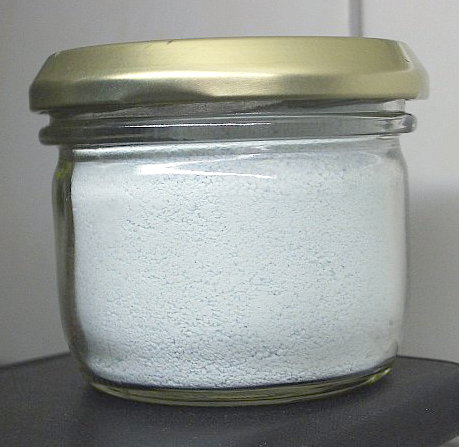
\includegraphics[width=\linewidth,height=4.2cm,keepaspectratio]{images/book1/cuso4-anhydrous.jpg}

{\small Le sulfate de cuivre anhydre~: une poudre blanche. Photo~:
W.~Oelen, CC BY-SA 3.0.}
\end{minipage}\hfill
\begin{minipage}[b]{0.48\linewidth}\centering
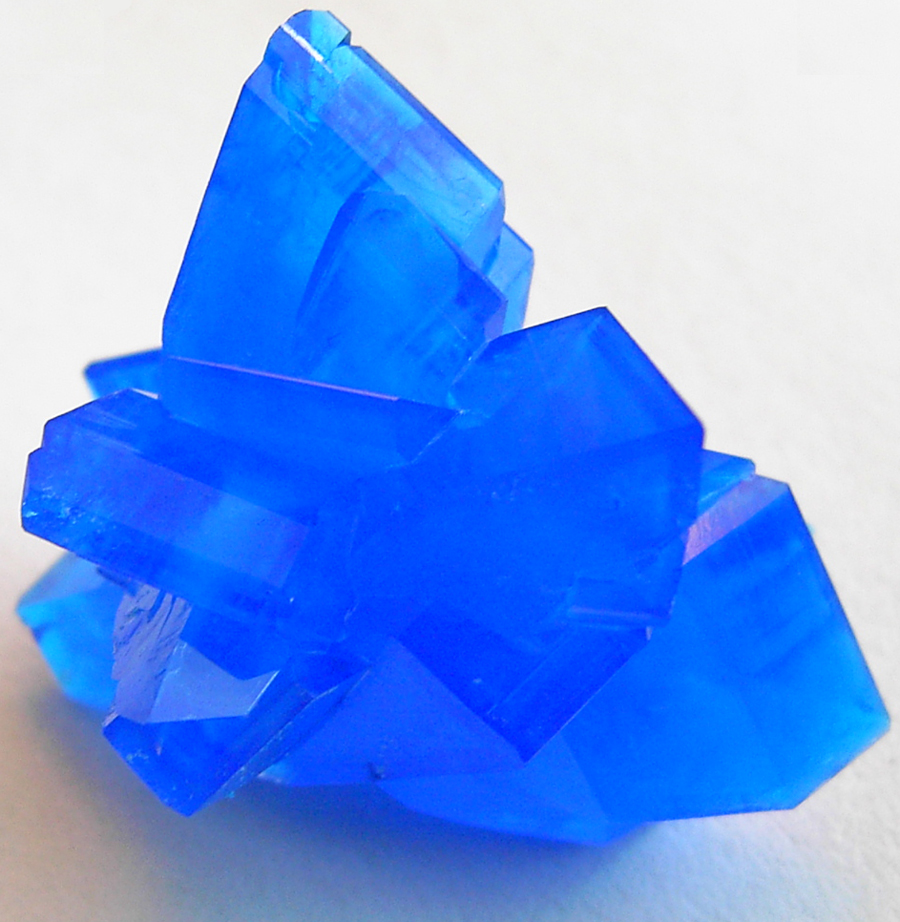
\includegraphics[width=\linewidth,height=4.2cm,keepaspectratio]{images/book1/cuso4-hydrated.jpg}

{\small Avec de l'eau, il bleuit~; ces cristaux contiennent de l'eau.
Photo~: Stephanb, CC BY-SA 3.0.}
\end{minipage}
\end{omfigure}

\begin{safety}{\ghs[0.82cm]{GHS05}\ghs[0.82cm]{GHS07}\ghs[0.82cm]{GHS09}}
% ledger: ghs:CuSO4
Le sulfate de cuivre est nocif en cas d'ingestion et irritant pour la
peau (GHS07)~; il peut gravement endommager les yeux (GHS05)~; il est
très toxique pour les organismes aquatiques, avec des effets durables
(GHS09). Lunettes et gants~; les déchets sont récupérés, jamais versés
dans l'évier.
\end{safety}

\begin{proposition}[Le dioxygène rallume une bûchette incandescente]\label{prop:g7:identifying-substances:splint}
On allume une bûchette de bois, puis on la souffle pour qu'il ne reste
qu'une lueur rouge. Plongée dans un tube à essai de dioxygène, la
bûchette incandescente se rallume en flamme.
\end{proposition}

\begin{proposition}[Le dihydrogène brûle avec une petite détonation]\label{prop:g7:identifying-substances:pop}
Une bûchette enflammée approchée de l'ouverture d'un petit tube à essai
de dihydrogène produit une petite détonation brève et aiguë, un
«~pop~»~: le dihydrogène \omterm{def:g4:what-a-fire-needs:burning}{brûle} aussitôt avec le dioxygène de l'\omterm{def:g4:air-a-mixture-of-gases:air}{air}.
\end{proposition}

\begin{omfigure}
\begin{tikzpicture}[font=\small, scale=1.25]
  % splint test for oxygen
  \pic[transform shape] at (0,0) {testtube={0}{white}};
  \draw[brown!60!black, line width=2pt] (0.15,1.6) -- (1.4,3.6);
  \fill[orange!85] (0.15,1.6) circle (0.07);
  \fill[orange!80] (0.12,1.62) .. controls (0.0,1.9) and (0.08,2.1) .. (0.1,2.3)
    .. controls (0.2,2.05) and (0.3,1.85) .. (0.2,1.62);
  \node[anchor=north, align=center] at (0,-0.15) {dioxygène~:\\ la bûchette\\ se rallume};
  % pop test for hydrogen
  \begin{scope}[xshift=4cm]
    \pic[transform shape, rotate=180] at (0,3.1) {testtube={0}{white}};
    \draw[brown!60!black, line width=2pt] (0.05,-0.05) -- (1.3,-0.9);
    \fill[orange!85] (0.05,-0.02) .. controls (-0.05,0.08) and (0.0,0.15) .. (0.02,0.22)
      .. controls (0.08,0.15) and (0.15,0.08) .. (0.1,-0.02);
    \node[font=\small\itshape] at (-0.9,0.15) {pop~!};
    \node[anchor=north, align=center] at (0,-1.0) {dihydrogène~:\\ un «~pop~» aigu\\ à l'ouverture};
  \end{scope}
\end{tikzpicture}

{\small À gauche~: une bûchette incandescente se rallume dans le
dioxygène. À droite~: une bûchette enflammée à l'ouverture d'un tube
retourné rempli de dihydrogène produit un «~pop~» aigu (le dihydrogène
est plus léger que l'\omterm{def:g4:air-a-mixture-of-gases:air}{air}, c'est pourquoi on tient le tube ouverture vers
le bas).}
\end{omfigure}

\begin{safety}{\ghs[0.82cm]{GHS02}\ghs[0.82cm]{GHS04}}
% ledger: ghs:H2
Le dihydrogène est un gaz extrêmement inflammable (GHS02), stocké sous
pression dans des bouteilles (GHS04). Le test du «~pop~» se fait avec
quelques millilitres seulement, par l'enseignant.
\end{safety}

\section{La chromatographie sur papier}

\begin{definition}[Chromatographie sur papier et chromatogramme]\label{def:g7:identifying-substances:chromatography}
La \emph{chromatographie sur papier}\index{chromatographie sur papier}
sépare les colorants d'un \omterm{def:g6:pure-substances-and-mixtures:mixture}{mélange}. On dépose une petite tache du \omterm{def:g6:pure-substances-and-mixtures:mixture}{mélange}
sur une ligne tracée près du bas d'une bande de papier~; le bas de la
bande trempe dans un \omterm{def:g6:solutions-and-solubility:solute}{solvant}, qui monte lentement le long du papier et
entraîne chaque colorant avec lui, certains plus vite que d'autres.
Quand le \omterm{def:g6:solutions-and-solubility:solute}{solvant} est monté presque jusqu'en haut, on retire la bande et
on la fait sécher~: c'est le
\emph{chromatogramme}\index{chromatogramme}.
\end{definition}

\begin{omfigure}
\begin{tikzpicture}[font=\small, scale=1.3]
  % the strip in a beaker of solvent
  \pic[transform shape] at (0,0) {beaker={0.12}{omWater!80}};
  \fill[white] (-0.42,0.06) rectangle (0.42,2.2);
  \fill[omWater!80] (-0.42,0.06) rectangle (0.42,0.24);
  \draw[omGlass, line width=0.6pt] (-0.42,0.06) rectangle (0.42,2.2);
  \draw[black!60, line width=0.4pt] (-0.42,0.42) -- (0.42,0.42);
  \fill[black!80] (0,0.42) circle (0.07);
  \shade[ball color=black!20] (0,2.27) circle (0.08);
  \draw[black!50, line width=1.2pt] (-1.1,2.27) -- (1.1,2.27);
  \node[anchor=north, align=center] at (0,-0.15) {au départ};
  \draw[<-, omProp, thick] (0.1,0.5) -- (1.3,0.8) node[right, text=black]
    {tache d'encre sur le trait};
  \draw[<-, omProp, thick] (1.0,2.27) -- (1.3,2.5) node[right, text=black]
    {baguette tenant le papier};
  \draw[<-, omProp, thick] (0.75,0.15) -- (1.3,0.25) node[right, text=black]
    {solvant, sous le trait};
  % the chromatogram
  \begin{scope}[xshift=6.2cm]
    \pic[transform shape] at (0,0) {tlcplate};
    \draw[black!50, dashed] (-0.7,2.7) -- (0.7,2.7);
    \fill[blue!70] (0,1.0) ellipse (0.13 and 0.09);
    \fill[red!70] (0,1.7) ellipse (0.13 and 0.09);
    \fill[yellow!80!orange] (0,2.35) ellipse (0.13 and 0.09);
    \node[anchor=north, align=center] at (0,-0.15) {le chromatogramme};
    \draw[<-, omProp, thick] (0.75,2.7) -- (1.3,2.85) node[right, text=black]
      {front du solvant};
    \draw[<-, omProp, thick] (0.2,1.7) -- (1.3,1.7) node[right, text=black]
      {trois colorants~: un mélange};
  \end{scope}
\end{tikzpicture}

{\small \omterm{def:g7:identifying-substances:chromatography}{Chromatographie sur papier} d'une encre noire. Le \omterm{def:g6:solutions-and-solubility:solute}{solvant} monte
dans le papier et sépare l'encre en trois colorants.}
\end{omfigure}

\begin{method}[Lire un chromatogramme]\label{met:g7:identifying-substances:read}
\begin{enumerate}
  \item Compter les taches au-dessus de chaque point de départ~: une
        tache, un colorant~; deux taches ou plus, un \omterm{def:g6:pure-substances-and-mixtures:mixture}{mélange} de colorants.
  \item Comparer les hauteurs~: sur un même \omterm{def:g7:identifying-substances:chromatography}{chromatogramme}, un colorant
        monte toujours à la même hauteur. Une tache à la même hauteur
        qu'un colorant connu est probablement ce colorant.
  \item Tracer le trait au crayon à papier, jamais à l'encre~: l'encre
        serait elle-même séparée par le \omterm{def:g6:solutions-and-solubility:solute}{solvant}.
\end{enumerate}
\end{method}

\begin{example}[Les colorants des bonbons]\label{ex:g7:identifying-substances:sweets}
On gratte l'enrobage coloré de bonbons dans un peu d'eau et on le dépose
sur une bande, à côté de taches des colorants alimentaires autorisés dans
les bonbons. Le \omterm{def:g7:identifying-substances:chromatography}{chromatogramme} montre que l'enrobage vert contient un
colorant jaune et un colorant bleu, tous deux parmi les colorants
autorisés.
\end{example}


\section{Lire une table de tests}

\begin{proposition}[Une table de tests caractéristiques]\label{prop:g7:identifying-substances:bank}
Les chimistes rassemblent les tests qu'ils utilisent dans un tableau, une
table de tests, qui se lit de gauche à droite~:
\begin{center}
\small
\begin{tabular}{llll}
\hline
espèce recherchée & \omterm{def:g7:identifying-substances:characteristic-test}{réactif} ou test & résultat positif & \\
\hline
dioxyde de carbone & eau de chaux & l'eau de chaux se trouble & \\
eau & sulfate de cuivre anhydre & le blanc devient bleu & \\
dioxygène & bûchette incandescente & la bûchette se rallume & \\
dihydrogène & bûchette enflammée & un «~pop~» aigu & \\
colorants d'un \omterm{def:g6:pure-substances-and-mixtures:mixture}{mélange} & \omterm{def:g7:identifying-substances:chromatography}{chromatographie sur papier} & une tache par colorant & \\
\hline
\end{tabular}
\end{center}
\end{proposition}

\begin{remark}[Ce qu'un test ne dit pas]\label{rem:g7:identifying-substances:limits}
Un test positif prouve que l'espèce est présente, pas qu'elle est
seule~: un liquide qui bleuit le sulfate de cuivre contient de l'eau,
mais ce peut être de l'eau salée ou du jus d'orange. Un test négatif dit
seulement que l'espèce est absente, ou présente en trop faible quantité
pour se manifester.
\end{remark}

\begin{omfigure}
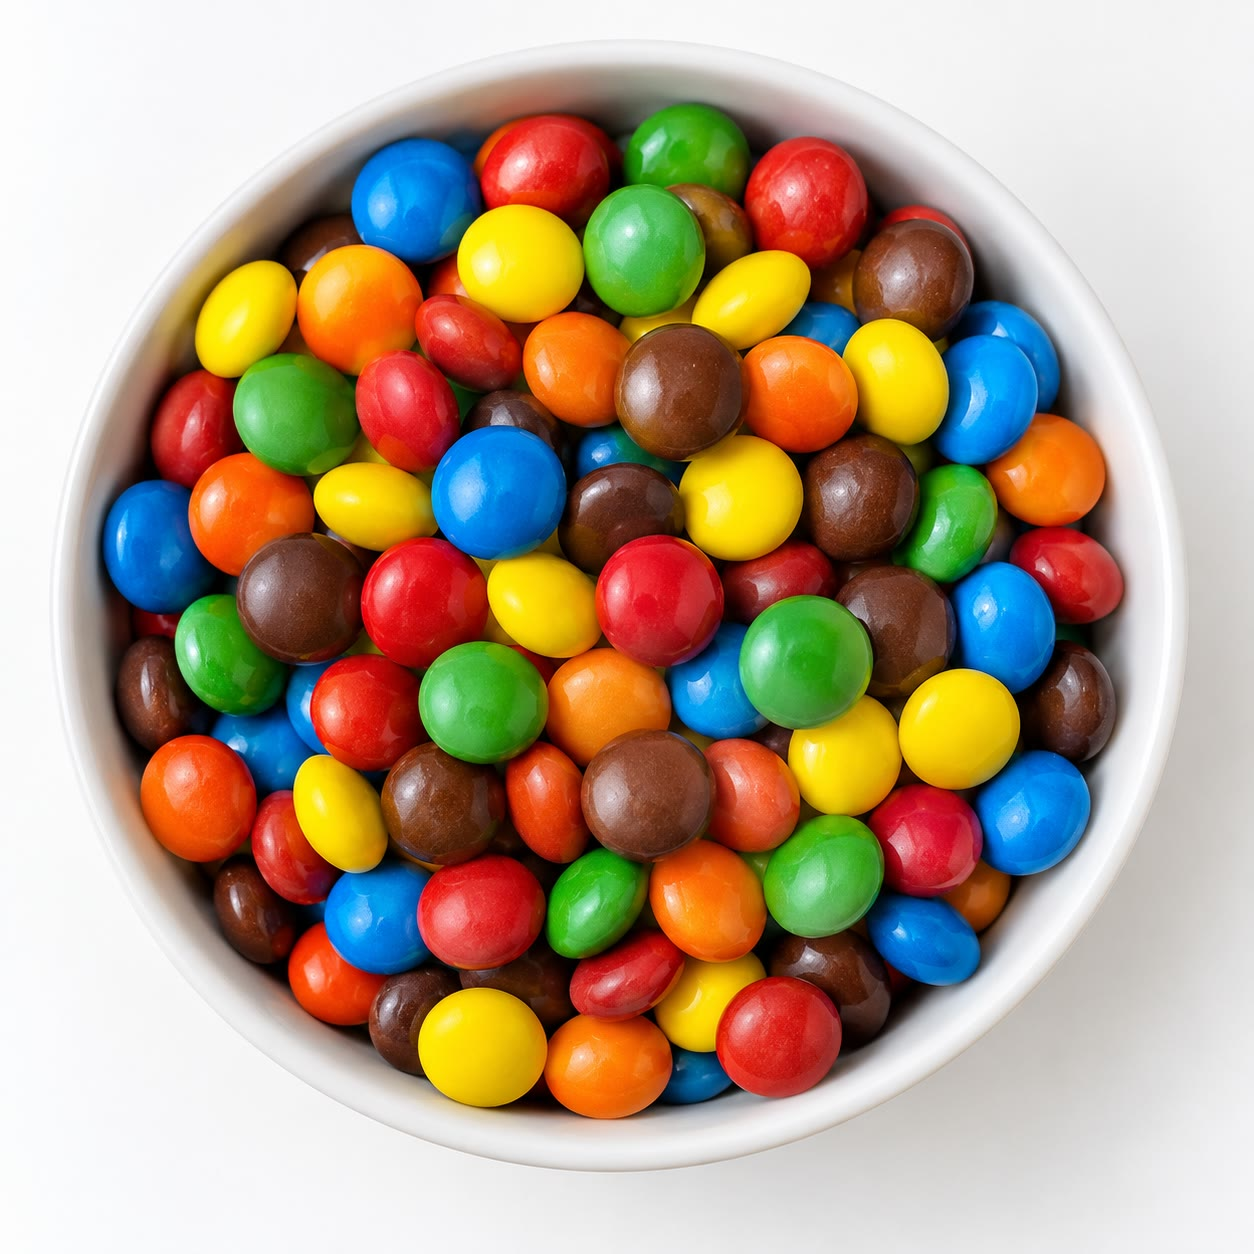
\includegraphics[width=0.32\linewidth]{images/book1/ai/g7-sweets.jpg}

{\small Des bonbons dragéifiés~: leurs couleurs sont des \omterm{def:g6:pure-substances-and-mixtures:mixture}{mélanges} de
colorants que la chromatographie peut séparer.}
\end{omfigure}

\begin{omfigure}
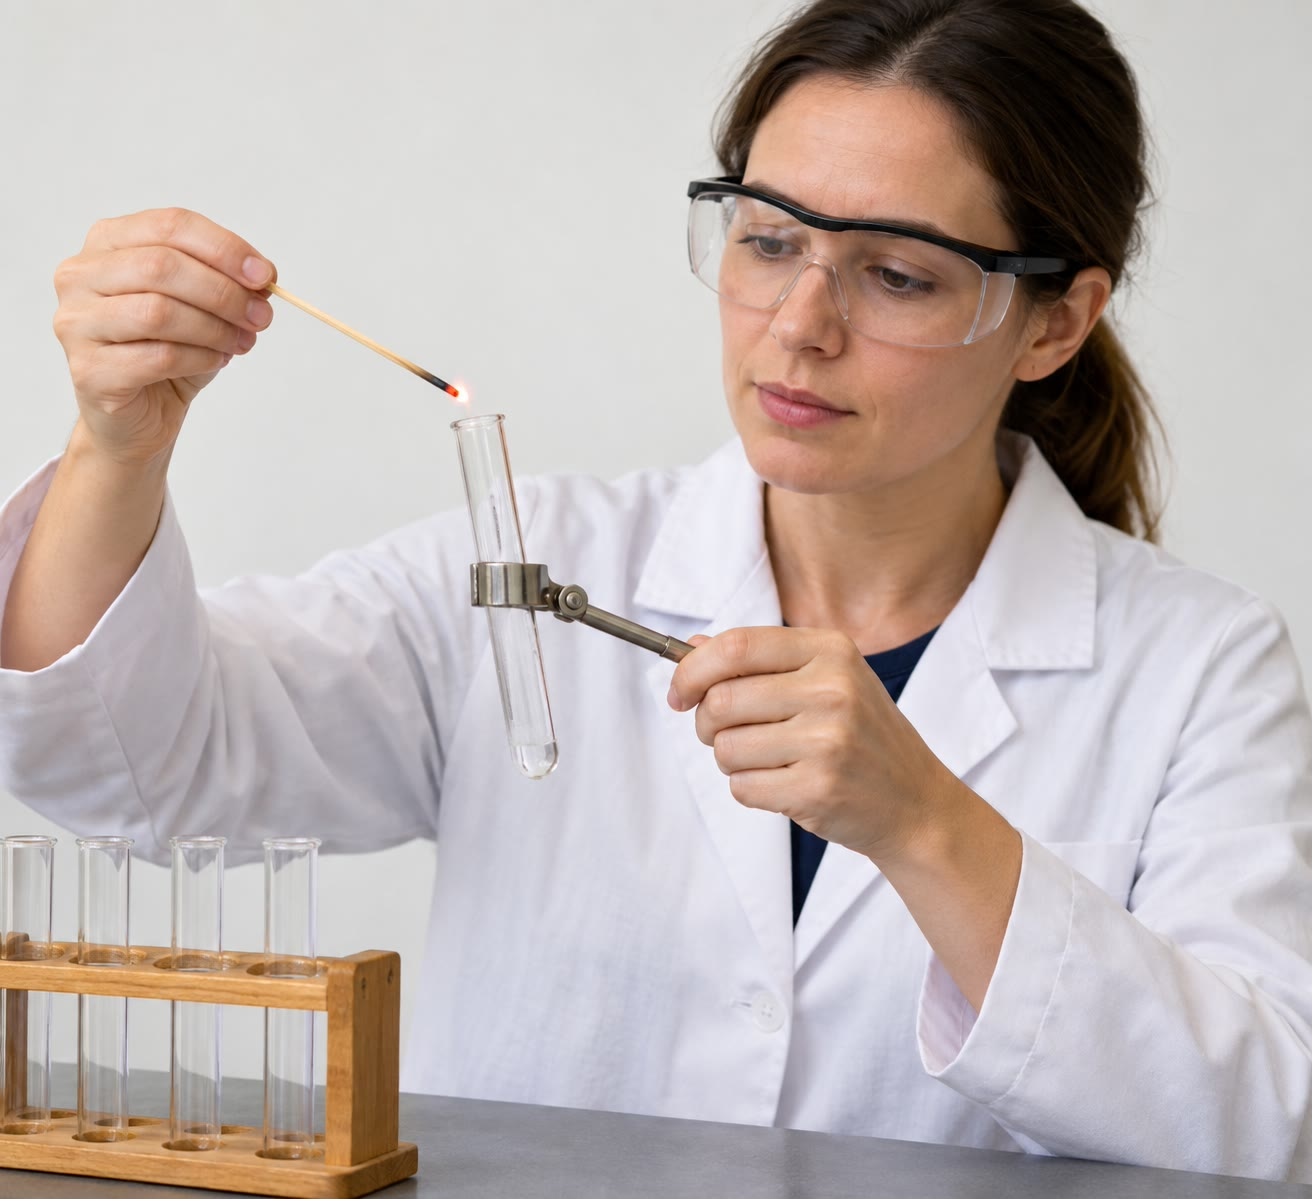
\includegraphics[width=0.36\linewidth]{images/book1/ai/g7-splint-teacher.jpg}

{\small Une enseignante teste un gaz avec une bûchette incandescente.}
\end{omfigure}

\section{Exercices}

\begin{exercise}[$\star$]\label{exo:g7:identifying-substances:1}
Quel test permet d'identifier le dioxyde de carbone~? Décris son
résultat positif.
\end{exercise}

\begin{exercise}[$\star$]\label{exo:g7:identifying-substances:2}
Une poudre blanche bleuit quand on y fait tomber un liquide. Que
montre ce résultat au sujet du liquide~?
\end{exercise}

\begin{exercise}[$\star$]\label{exo:g7:identifying-substances:3}
On plonge une bûchette incandescente dans un flacon de gaz, et elle se
rallume en flamme. Quel gaz le flacon contient-il~?
\end{exercise}

\begin{exercise}[$\star$]\label{exo:g7:identifying-substances:4}
Pourquoi trace-t-on la ligne de départ d'un \omterm{def:g7:identifying-substances:chromatography}{chromatogramme} sur papier au
crayon à papier et non à l'encre~?
\end{exercise}

\begin{exercise}[$\star\star$]\label{exo:g7:identifying-substances:5}
Pourquoi la ligne de départ doit-elle se trouver au-dessus du niveau du
\omterm{def:g6:solutions-and-solubility:solute}{solvant} dans le bécher~?
\end{exercise}

\begin{exercise}[$\star\star$]\label{exo:g7:identifying-substances:6}
Le \omterm{def:g7:identifying-substances:chromatography}{chromatogramme} d'une encre verte montre deux taches, l'une à la
hauteur d'un colorant jaune de référence, l'autre à la hauteur d'un
colorant bleu de référence. L'encre verte est-elle un \omterm{def:g6:pure-substances-and-mixtures:pure-substance}{corps pur}~? De
quoi est-elle faite~?
\end{exercise}

\begin{exercise}[$\star\star$]\label{exo:g7:identifying-substances:7}
À l'aide de la table de tests, quel test utiliserais-tu pour montrer
qu'un gaz dégagé par une réaction est du dihydrogène~? Qu'attends-tu
d'observer~?
\end{exercise}

\begin{exercise}[$\star\star$]\label{exo:g7:identifying-substances:8}
L'\omterm{def:g4:air-a-mixture-of-gases:air}{air} expiré trouble l'eau de chaux bien plus vite que l'\omterm{def:g4:air-a-mixture-of-gases:air}{air} frais. Que
nous apprend ce résultat sur l'\omterm{def:g4:air-a-mixture-of-gases:air}{air} que nous expirons~?
\end{exercise}

\begin{exercise}[$\star\star$]\label{exo:g7:identifying-substances:9}
Un liquide limpide bleuit le sulfate de cuivre anhydre. Sam conclut~:
«~C'est de l'eau pure.~» Explique pourquoi Sam se trompe.
\end{exercise}

\begin{exercise}[$\star\star$]\label{exo:g7:identifying-substances:10}
Regarde le \omterm{def:g7:identifying-substances:chromatography}{chromatogramme} de l'encre noire dans ce chapitre. Combien de
colorants l'encre contient-elle~? Lequel est monté le plus haut~?
\end{exercise}

\begin{exercise}[$\star\star\star$]\label{exo:g7:identifying-substances:11}
Trois flacons contiennent du dioxygène, du dihydrogène et du dioxyde de
carbone, mais leurs étiquettes sont perdues. Prévois, sur le papier, les
tests qui permettraient de nommer chaque flacon, dans un ordre qui
utilise le moins de tests possible.
\end{exercise}

\begin{exercise}[$\star\star\star$]\label{exo:g7:identifying-substances:12}
Un élève teste un gaz avec de l'eau de chaux et ne voit rien se passer.
Donne deux explications possibles, et le témoin qui aiderait à
trancher.
\end{exercise}

\section{Problème~: le mot falsifié}

\begin{problem}[{Problème du week-end --- un mot écrit au feutre, trois
feutres suspects, trois bouteilles de gaz sans étiquette, et une table de
tests}]
\label{pb:g7:identifying-substances:1}
Un laboratoire scolaire est appelé à l'aide pour deux petites énigmes.
D'abord, un mot écrit au feutre noir doit être attribué à l'un de trois
feutres noirs, 1, 2 et 3. On prélève une goutte d'encre sur le mot et sur
chaque feutre, et on les dépose sur une même bande de papier, que l'on
développe ensuite avec de l'eau. Le \omterm{def:g7:identifying-substances:chromatography}{chromatogramme} est représenté
ci-dessous.
\begin{center}
\begin{tikzpicture}[font=\small, x=1cm, y=1cm]
  \fill[white] (0,0) rectangle (6,4);
  \draw[omGlass, line width=0.6pt] (0,0) rectangle (6,4);
  \draw[black!60] (0,0.5) -- (6,0.5);
  \draw[black!50, dashed] (0,3.6) -- (6,3.6);
  \foreach \x/\lab in {0.9/mot, 2.3/feutre 1, 3.7/feutre 2, 5.1/feutre 3}
    \node[anchor=north] at (\x,-0.05) {\lab};
  % note: three dyes
  \fill[blue!70] (0.9,1.2) ellipse (0.18 and 0.1);
  \fill[red!70] (0.9,2.2) ellipse (0.18 and 0.1);
  \fill[yellow!80!orange] (0.9,3.1) ellipse (0.18 and 0.1);
  % pen 1: two dyes
  \fill[blue!70] (2.3,1.2) ellipse (0.18 and 0.1);
  \fill[black!70] (2.3,2.7) ellipse (0.18 and 0.1);
  % pen 2: same three as the note
  \fill[blue!70] (3.7,1.2) ellipse (0.18 and 0.1);
  \fill[red!70] (3.7,2.2) ellipse (0.18 and 0.1);
  \fill[yellow!80!orange] (3.7,3.1) ellipse (0.18 and 0.1);
  % pen 3: three dyes, other heights
  \fill[violet!70] (5.1,0.9) ellipse (0.18 and 0.1);
  \fill[red!70] (5.1,1.8) ellipse (0.18 and 0.1);
  \fill[green!60!black] (5.1,2.6) ellipse (0.18 and 0.1);
  \node[anchor=west, font=\footnotesize] at (6.1,3.6) {front du solvant};
  \node[anchor=west, font=\footnotesize] at (6.1,0.5) {ligne de départ};
\end{tikzpicture}
\end{center}

\medskip
\noindent\textbf{Partie I --- Le \omterm{def:g7:identifying-substances:chromatography}{chromatogramme}.}
\begin{enumerate}
  \item Pourquoi a-t-on déposé les quatre encres sur la même bande et
        les a-t-on développées ensemble~?
  \item L'encre du mot est-elle un \omterm{def:g6:pure-substances-and-mixtures:pure-substance}{corps pur} ou un \omterm{def:g6:pure-substances-and-mixtures:mixture}{mélange}~? Explique.
  \item Combien de colorants l'encre du feutre 1 contient-elle~? Le
        feutre 1 peut-il avoir écrit le mot~?
  \item Le feutre 3 contient lui aussi trois colorants. Pourquoi ne
        peut-il pas avoir écrit le mot~?
  \item Quel feutre correspond au mot~? Explique à l'aide des hauteurs
        des taches.
\end{enumerate}

\medskip
\noindent\textbf{Partie II --- Trois bouteilles de gaz.}
Seconde énigme~: trois petites bouteilles, X, Y et Z, ont perdu leurs
étiquettes~; elles contiennent du dioxygène, du dihydrogène et du
dioxyde de carbone. On recueille un peu de gaz de chacune dans un tube à
essai. Le gaz X rallume une bûchette incandescente. Le gaz Y produit un
«~pop~» aigu avec une bûchette enflammée. Le gaz Z trouble l'eau de
chaux.
\begin{enumerate}[resume]
  \item Nomme le gaz X.
  \item Nomme le gaz Y.
  \item Nomme le gaz Z.
  \item Avant de tester le gaz Z, l'élève fait barboter de l'\omterm{def:g4:air-a-mixture-of-gases:air}{air} ordinaire
        dans la même eau de chaux pendant le même temps, et elle reste
        limpide. Comment s'appelle ce second essai, et qu'ajoute-t-il à
        la conclusion~?
\end{enumerate}

\medskip
\noindent\textbf{Partie III --- La table de tests.}
\begin{enumerate}[resume]
  \item Un liquide incolore trouvé à côté du mot bleuit le sulfate de
        cuivre anhydre. Écris la ligne de la table de tests utilisée, et
        ce que montre le résultat.
  \item Ce résultat prouve-t-il que le liquide est de l'eau pure~?
        Explique.
  \item Conclus la première énigme~: combien de colorants l'encre du mot
        contient-elle, et quel feutre l'a écrit~?
\end{enumerate}
\end{problem}
